% last updated in April 2002 by Antje Endemann
% Based on CVPR 07 and LNCS, with modifications by DAF, AZ and elle, 2008 and AA, 2010, and CC, 2011

\documentclass[runningheads]{llncs}
\usepackage{graphicx}
\usepackage[font=small]{caption}
\usepackage{subcaption}
\captionsetup{compatibility=false}
\usepackage{amsmath,amssymb} % define this before the line numbering.
\usepackage{ruler}
\usepackage{color}
\usepackage{url}
\usepackage[width=122mm,left=12mm,paperwidth=146mm,height=193mm,top=12mm,paperheight=217mm]{geometry}
\usepackage{multirow}
\usepackage{tabularx}
\setlength{\extrarowheight}{2pt}
\newcolumntype{Y}{>{\centering\arraybackslash}X}
\captionsetup[table]{belowskip=12pt,aboveskip=4pt}
\setlength{\floatsep}{7pt plus 2pt minus 2pt}
\setlength{\textfloatsep}{7pt plus 2pt minus 2pt}
\setlength{\intextsep}{7pt plus 2pt minus 2pt}

\begin{document}
% \renewcommand\thelinenumber{\color[rgb]{0.2,0.5,0.8}\normalfont\sffamily\scriptsize\arabic{linenumber}\color[rgb]{0,0,0}}
% \renewcommand\makeLineNumber {\hss\thelinenumber\ \hspace{6mm} \rlap{\hskip\textwidth\ \hspace{6.5mm}\thelinenumber}}
% \linenumbers \

\pagestyle{headings}
\mainmatter
\def\ECCV14SubNumber{150}  % Insert your submission number here

\title{A Motion Blur Resilient Fiducial Marker For Quadcopter Imaging} % Replace
% with your title

\titlerunning{ECCV-14 submission ID \ECCV14SubNumber}

\authorrunning{ECCV-14 submission ID \ECCV14SubNumber}

\author{Anonymous ECCV submission}
\institute{Paper ID \ECCV14SubNumber}

\maketitle

\begin{abstract}
This paper describes the design and evaluation of a binary fiducial marker
design for use with low-cost quadcopters.  Fiducial markers are commonly placed
into environments to provide a reliable and unique scene marker conducive for
tracking and recognition.   For quadcopter applications, fiducials are
typically used for evaluating planning algorithms by allowing ground truth
positions in the scene to be detected from the quadcopter's camera. Quadcopters,
however, are subject to quick and unstable motions that causes notable motion
blur that severely affects the detection rate of existing fiducial markers. 
This motivated us to design a fiducial that is robust to motion blur. Our design
uses a series of concentric circles with the observation is that the direction
perpendicular to the motion blur direction will be unaffected by the blur and
therefore still be recognized as a binary code.  We detail the design and
detection algorithm for our fiducial and show that our marker can significantly
outperform existing fiducials on scenes captured with a quadcopter.
\keywords{Fiducials, Tracking, Detection using Blur}
\end{abstract}

\section{Introduction}
Recently, use of Unmanned Aerial Vehicles(UAV) such as quadcopters is increased
in various tracking activities e.g. aerial surveillance, search and rescue
operations etc. Navigation of these vehicles is mainly based on the
onboard inertial sensors. But sensor based measurments are prone to errors. So,
visual cues captured through onboard camera can be used along with the sensor
based measurments.  But, natural features may not be available always and
quality cannot be guaranteed in every scene. So, results are not satisfactory in
uncontrolled environment and hence use of such features is limited specifically
when we need very high precision.

Artificial markers are used when we need high precision. A fiducial marker or
simply a fiducial is an synthetic object placed in the scene, which can provide
additional information about the environment. Artificial fiducials are widely
used in Augmented Reality(AR) \cite{Zhang:2002}\cite{Dorfmuller99}
applications, vision based navigation of robots\cite{Davison:2007} etc.

Low cost quadcopters such as AR Drone are very unstable which
causes non-uniform motion resulting lot of motion blur in captured images.
Also, as image transfer is done through wireless media using User Datagram
Protocol (UDP), there is possibility of missing intermediate frames . It
results in lower frame rate (around 15 frames per second (FPS)) instead of
normal rate of 30 FPS. This frequent dropping of frames may cause drastic
change in position of object in successive frames. Thus, performance of
traditional tracking methods is not satisfactory for tracking through
quadcopters. Our aim is to design a fiducial which we will be able to track
under significant amount of motion blur and is robust in terms of drastic
change in its position in successive frames.

We observed that blur in a single frame captured through quadcopter is linear.
There is no blur in the direction perpendicular to the direction of motion. We
tried to design a fiducial whose ``signature'' remains intact in any direction.

\begin{figure}
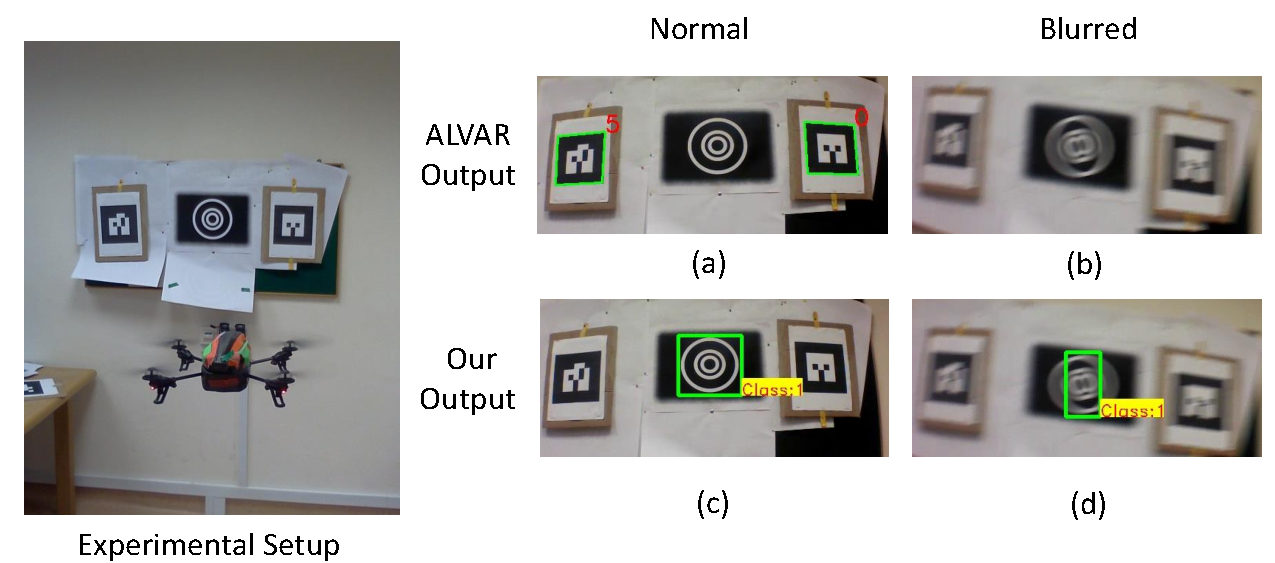
\includegraphics[width=\linewidth]{teaser.pdf}
\caption{Figure showing experimental setup and comparison of
output of ALVAR\cite{alvar} (for detecting ARTag) versus output of our
algorithm, in normal and blurred scene}
\end{figure}

\section{Related Work}
Our work is related to two areas: fiducial markers and
object tracking. We will briefly discuss work done in both areas.
\begin{figure}
 \begin{subfigure}[b]{0.19\textwidth}
  \centering
  
\includegraphics[width=\linewidth]{intersense.jpg}
  Intersense\cite{NaimarkF02}
 \end{subfigure}
 \begin{subfigure}[b]{0.19\textwidth}
 \centering
  
\includegraphics[width=\linewidth]{pattKanji.pdf}
  ARToolkit\cite{ARToolkit02}
 \end{subfigure}
 \begin{subfigure}[b]{0.19\textwidth}
  \centering
  
\includegraphics[width=\linewidth]{ARtag.jpg}
  ARTag\cite{Fiala05}
 \end{subfigure}
 \begin{subfigure}[b]{0.19\textwidth}
  \centering
  
\includegraphics[width=\linewidth]{pifiducial.png}
  Pi-Tag\cite{Pitag13}
 \end{subfigure}
 \begin{subfigure}[b]{0.19\textwidth}
  \centering
  
\includegraphics[width=\linewidth]{our_fiducial}
  Our Fiducial
 \end{subfigure}
 \caption{Various Fiducial Marker Designs}
 \label{fig:previous_work}
\end{figure}

The ARToolkit \cite{ARToolkit02} \cite{kato-artoolkit} is well known toolkit in
Augmented Reality system, widely used to find pose of the object on which it is
placed.  Fiala et al. \cite{Fiala05} developed a fiducial termed, ARTag, which is a
bi-tonal system consisting of a square border and
an interior region filled with a 6x6 grid of black or white cells. It proved to
be more efficient than \cite{ARToolkit02} in terms of marker recognition rate
as well as the number of different patterns which can be created.

Concentric rings are reportedly used first by Gatrell et al.\cite{concentric}
for monocular pose estimation as well as object identification in space. Cho et al.
\cite{Cho:2001}\cite{Cho97fastcolor} have used multi color rings in wide area
tracking in large scale applications. In \cite{NaimarkF02}, Naimark et al.
have developed ``Circular Data Matrix Fiducial System'', for wide area tracking.

Zhang el. al.\cite{Zhang:2002} and Claus et al. \cite{ClausF04} have done
quite comprehensive comparative study of various fiducial marker systems with
respect to processing time, recognition rate and accuracy with
respect to viewing angle and distance.

Bergamasco et al. \cite{runetag11} developed RUNE-Tag, fiducial marker
system which works under large amount of occlusion. Bergamasco et al. also
designed Pi-Tag \cite{Pitag13}, marker design based on projective
invariants.

The main hurdle in detection of current fiducials is, the detecton of features:
lines in \cite{ARToolkit02}, corners in \cite{Fiala05} while ellipses in
\cite{Cho:2001}, \cite{Cho97fastcolor}, \cite{runetag11} and \cite{Pitag13}.
Such features are very difficult to detect accurately under significant motion
blur. So, under blur, recognition rate of these fiducials is very low.

Fiducial detection in video may be considered as tracking problem where tracked
object is fiducial itself. Visual tracking plays an important role in
surveillance, robotics, human computer interaction, and medical
imaging\cite{Yilmaz:2006}. Yilmaz et al.\cite{Yilmaz:2006} have done survey of
various tracking methods. Most tracking methods
( \cite{Ross:2008} \cite{Wu:2009} \cite{Perez02} \cite{Mei:2009} ) assume image
sequence to be blur free. But in reality, motion blur is inherent part of most
of the videos. Wu et al.\cite{Wu:2011} have developed BLUr-driven Tracker (BLUT)
framework for tracking motion-blurred targets. BLUT is based on the observation
that although motion blurs degrade the visual features of the target, they, at
thde same time, provide useful cues about the movements to help tracking.

BLUT framework successfully tracks blurred target when there is uniform motion
and the position of tracked object does not change drastically in successive
frames. But in our case, due to frequntly dropping of intermediate frame, this
criterion may not be satisfied.

\section{Design of Fiducial}

Before we detail the design of our fiducial, we examine the performance of two
popular fidicuals, ARTags and PiTags, in the face of motion blur.

We conducted a small experiment to test ARTag's resilience towards blur.
We scaled down ARTag fiducial to size 150x150.  Then, we blurred ARTag
at various orientations using different scales. Finally, we tried to detect
ARTag in these blurred images using ALVAR library\cite{alvar}.

\begin{minipage}{\textwidth}
  \begin{minipage}[b]{0.49\textwidth}
\captionof{table}{Recognition rate of AR Tag at various blur scales}
\centering
 \begin{tabularx}{0.75\textwidth}{|Y|Y|}
\cline{1-2}
Blur Scale & Recognition Rate(\%) \\ \cline{1-2}
30 & 100\\ \cline{1-2}
35 & 19 \\ \cline{1-2}
40 & 9 \\ \cline{1-2}
45 & 5 \\ \cline{1-2}
50 & 0 \\ \cline{1-2}
\end{tabularx}
\label{tab:ARTag_blur}
 \end{minipage}	
 \begin{minipage}[b]{0.49\textwidth} 	
\captionof{table}{Blur angle range}
\centering
\begin{tabularx}{0.75\textwidth}{|Y|Y|}
\cline{1-2}
Blur Scale & Blur Angle Range \\ \cline{1-2}
30 & 0 -- 90\\ \cline{1-2}
35 & 32 -- 58 \\ \cline{1-2}
40 & 41 -- 48 \\ \cline{1-2}
45 & 41 -- 48 \\ \cline{1-2}
50 & 44 -- 46 \\ \cline{1-2}
\end{tabularx}
\label{tab:artag_blurangle}
 \end{minipage}
\end{minipage}

From Table \ref{tab:ARTag_blur}, it can be clearly seen that performance of
ARTag drastically degrade with increase in blur scale.

We have also analysed the recognition rate along different blur orientations
(from 0 to 90 degrees) at different blur scales. We found that per blur scale,
at certain blur orientations, recognition of ARTag fails. Table shows the range
of blur angles for which we are able to recognise the ARTag at different blur
scales. From Table \ref{tab:artag_blurangle}, it can be seen that, when blur
scale is greater than 30, ARTag is not recognisable with horizontal blur
orientation(blur angle near zero degrees) as well as vertial blur
orientation(blur angle near 90 degrees).

\begin{figure}
\centering
  
\includegraphics[width=.22\linewidth]{newconcentric_00.pdf}
  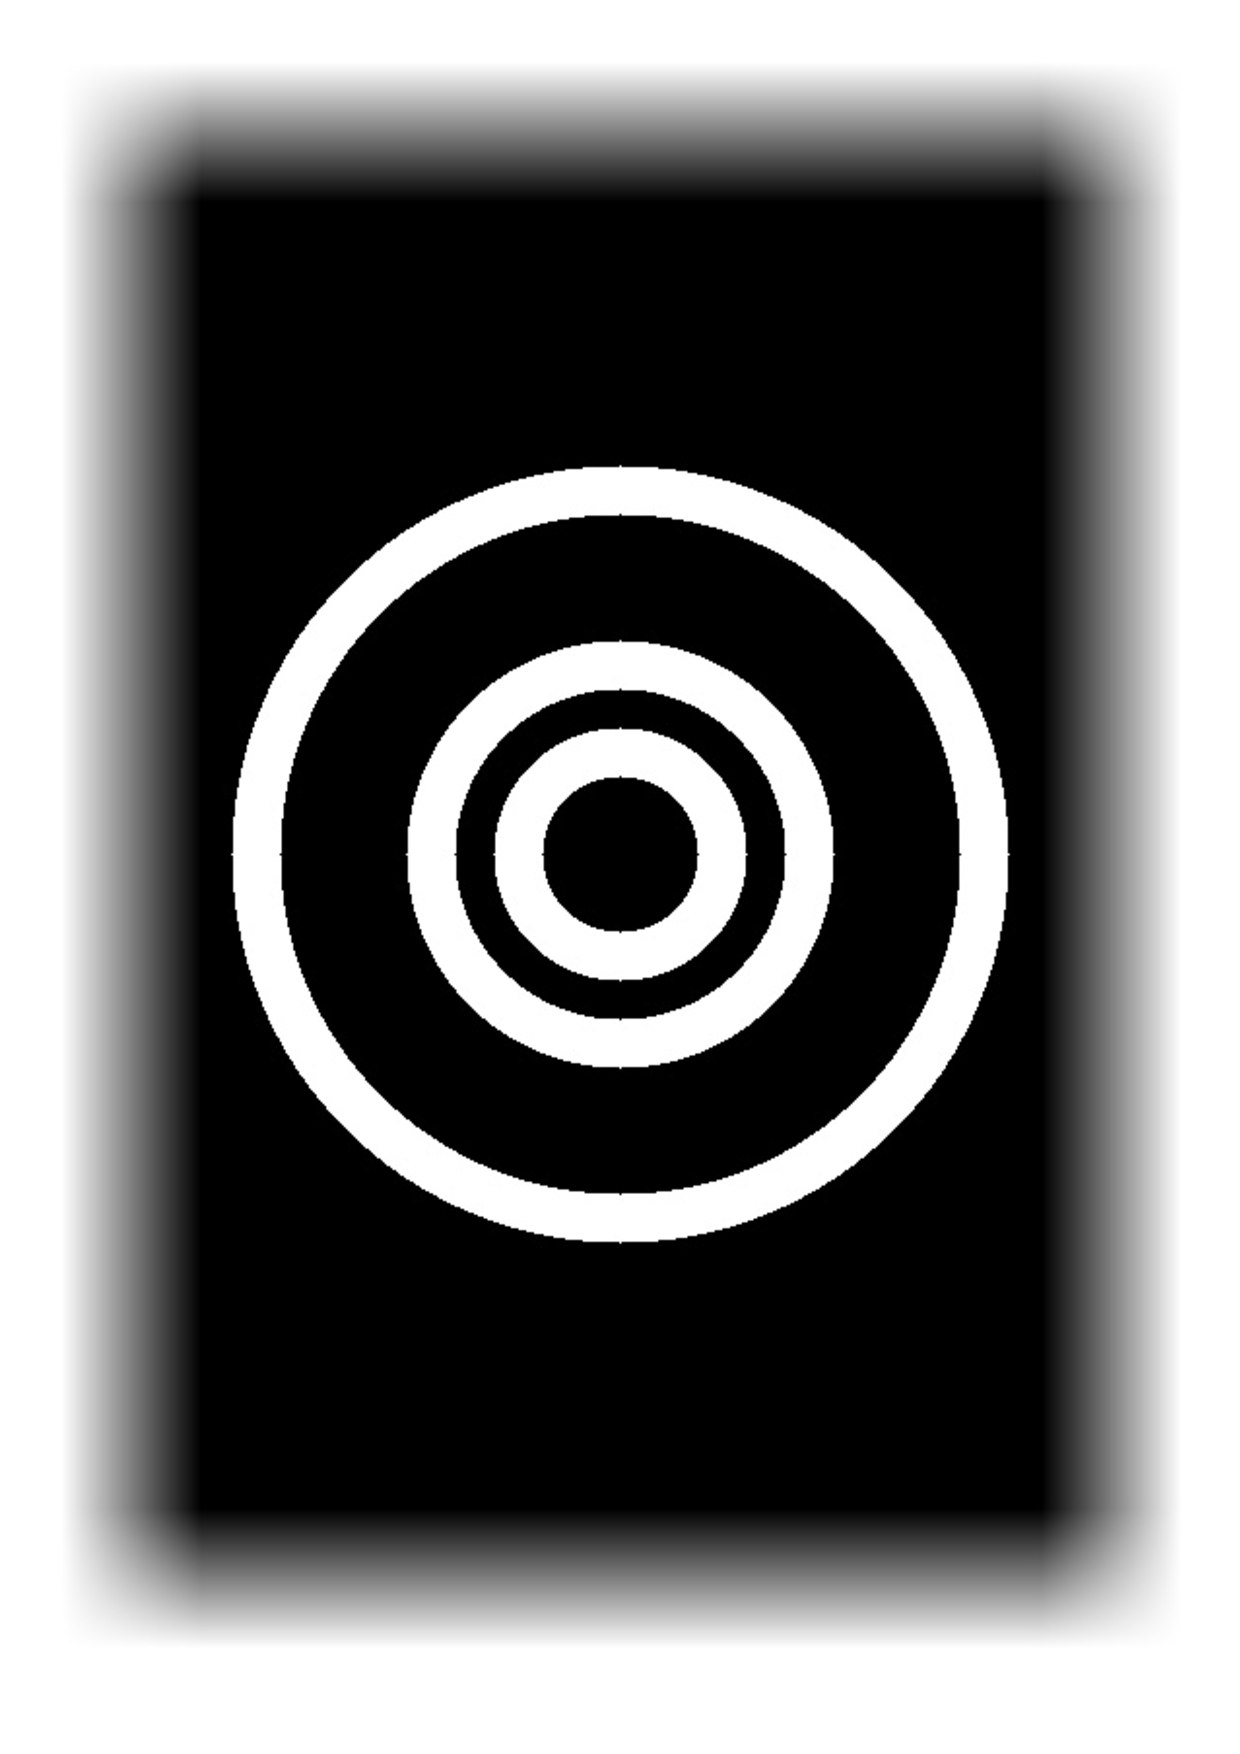
\includegraphics[width=.22\linewidth]{newconcentric_01.pdf}
  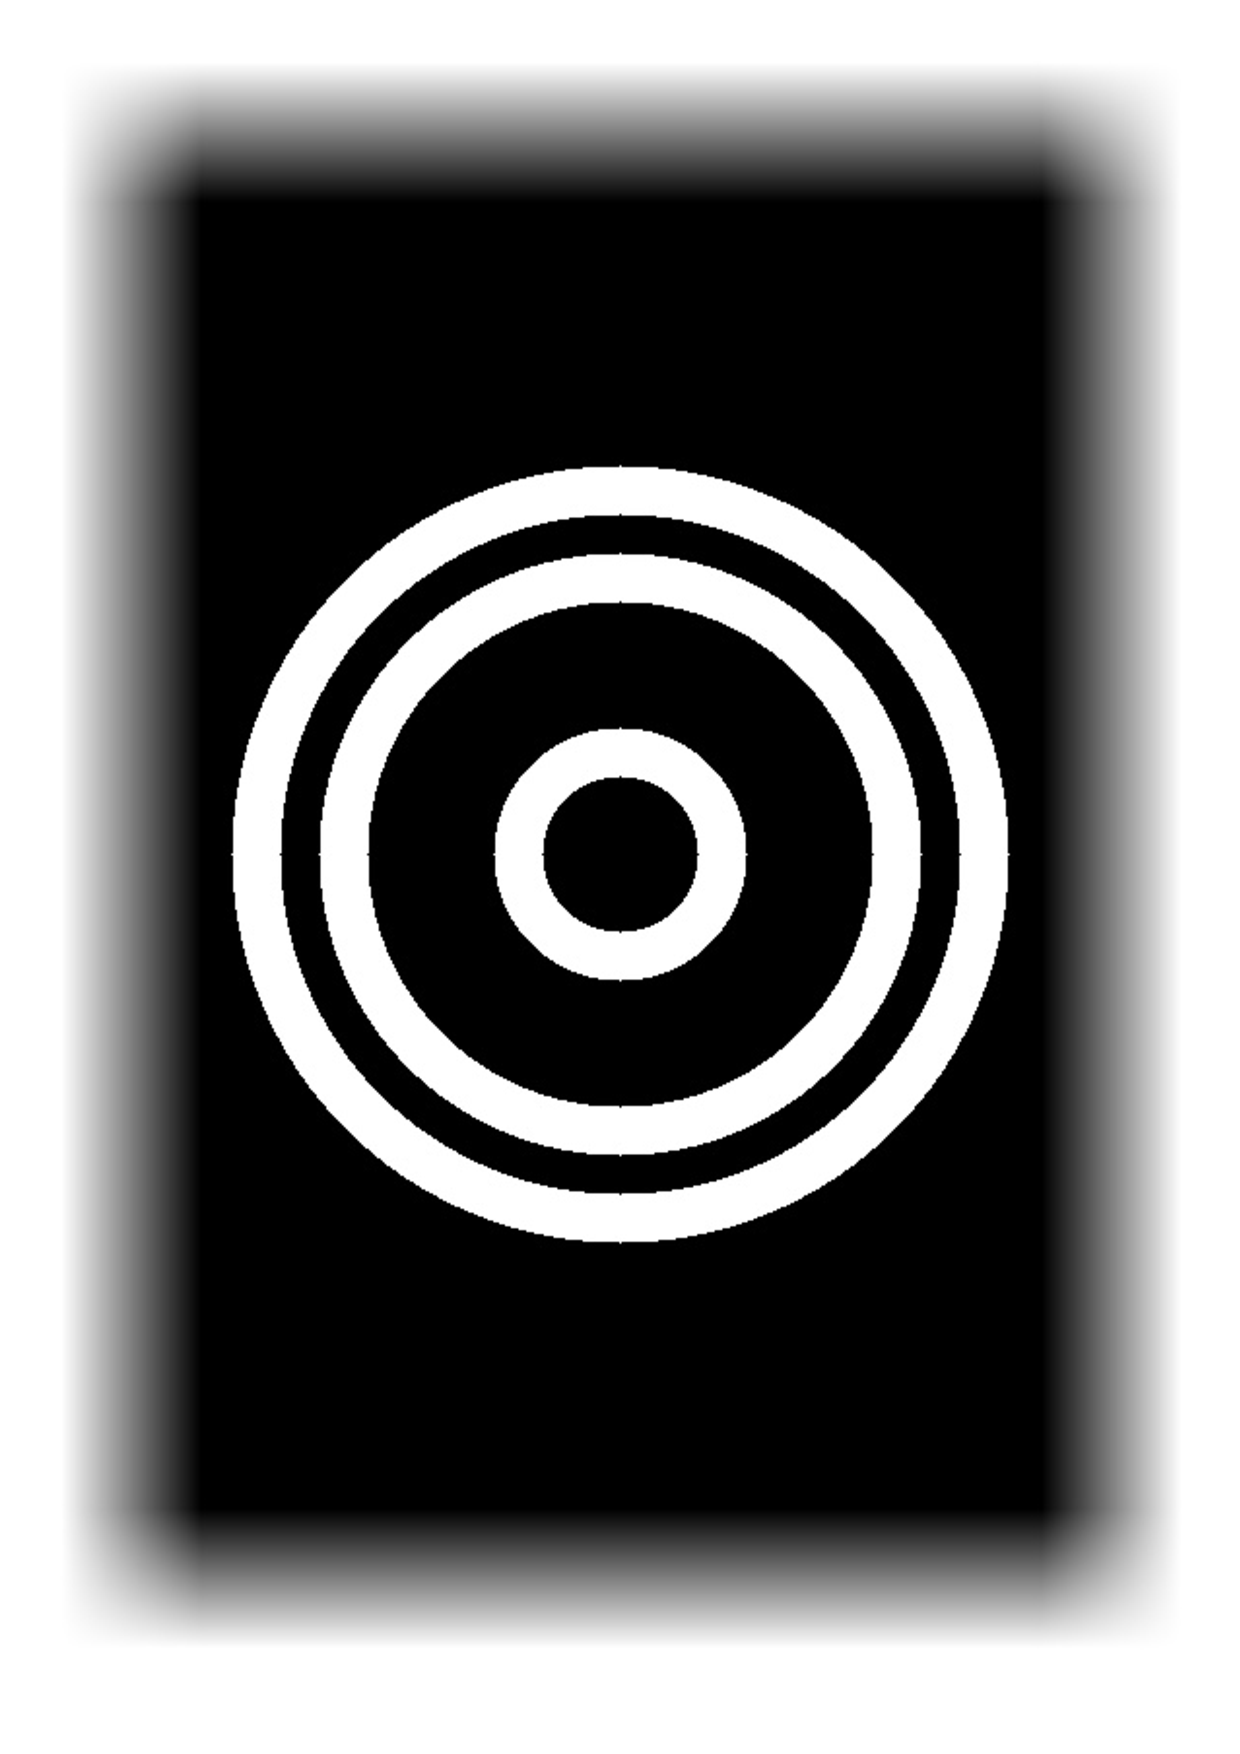
\includegraphics[width=.22\linewidth]{newconcentric_10.pdf}
  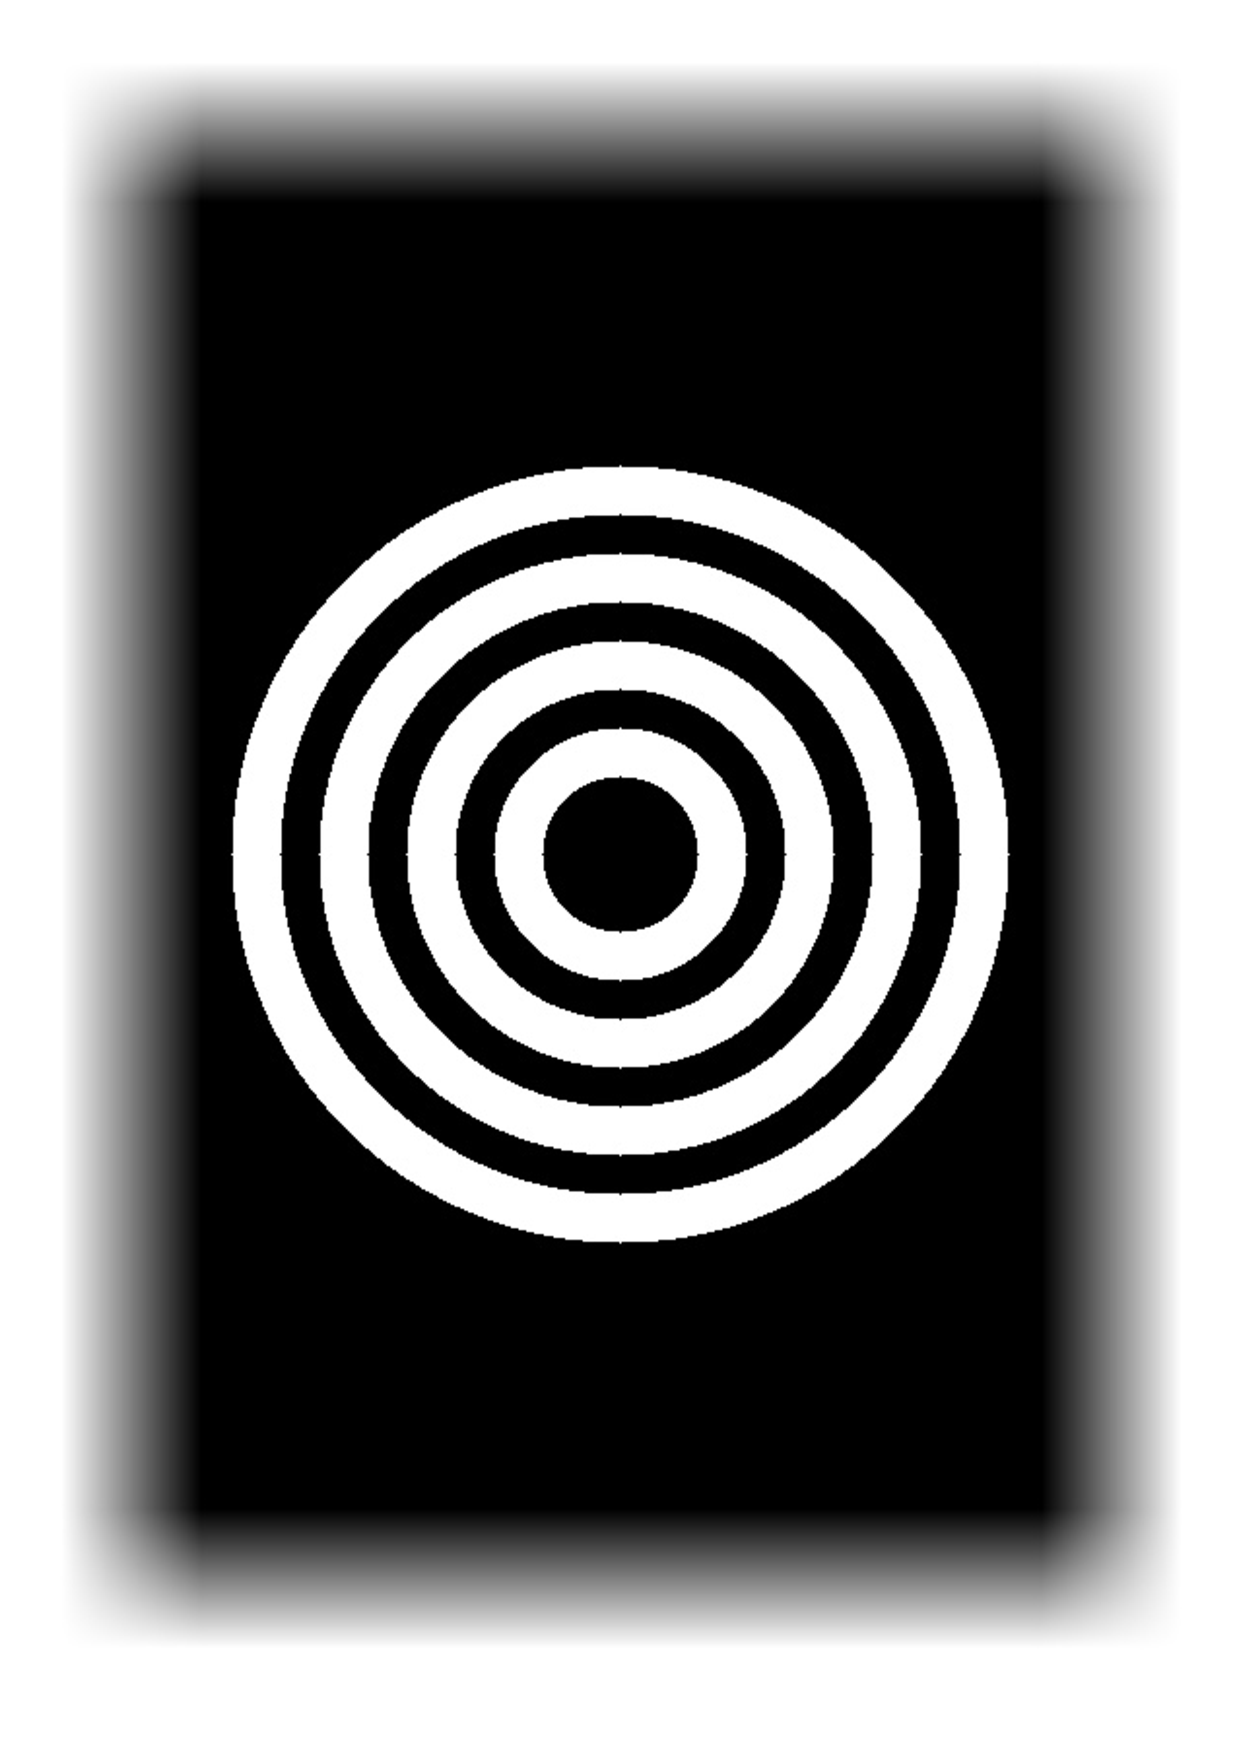
\includegraphics[width=.22\linewidth]{newconcentric_11.pdf}
  \caption{Two bit binary coded Fiducials (from left to right: Binary Code 00,
  Binary Code 01, Binary Code 10, Binary Code 11)}
  \label{fig:fiducials}
\end{figure}

Inspired from Circular Data Matrix\cite{NaimarkF02} we have designed a fiducial
that may be thought of as a binary code.  It contains concentric white rings of
equal widths on a black background with a blurred border. The outermost and
innermost rings represent the start and end of the code and is embedded in the
fiducial; these are not considered part of the code itself. The binary code is
represented by the presence (or absence) of rings between ``marker'' rings.

Depending on which ring is present or absent, the resulting binary code will
change. The number of different patterns depends on the number of bits in the
binary code. For example, if the binary code has three bits, there will be a
maximum of three rings between``marker'' rings and we end up with eight
different patterns. Fig. \ref{fig:fiducials} shows two bit binary coded
fiducials.

\section{Fiducial Detection Algorithm}

We have performed blur simulation experiment on Pi-tag \cite{Pitag13} to find
how blur effects circular patterns. We tried to detect blurred Pi-tag using
\cite{ros_pitag}.

\begin{figure}
\begin{subfigure}[b]{0.3\textwidth}
  \centering
  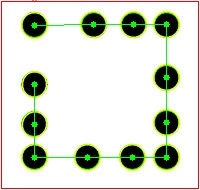
\includegraphics[width=\linewidth]{detect_noblur.jpg}
  No Blur  
 \end{subfigure}
 \begin{subfigure}[b]{0.3\textwidth}
  \centering
  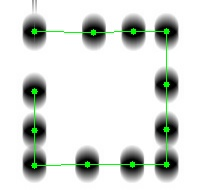
\includegraphics[width=\linewidth]{detect_blur15.jpg}
  Blur Scale = 15  
 \end{subfigure}
 \begin{subfigure}[b]{0.3\textwidth}
  \centering
  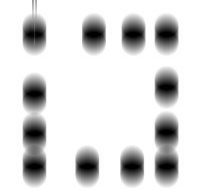
\includegraphics[width=\linewidth]{nodetect_blur20.jpg}
  Blur Scale = 20  
 \end{subfigure}
 \caption{Effect of blur on detection of Pi-Tag}
 \label{fig:pitag_blur}
\end{figure}

From Fig. \ref{fig:pitag_blur}, it can be seen that, Pi-tag detection
fails when blur scale is more than 15. The reason behind this is, Pi-tag
detection is based on Ellipse detection which will fail in the presence of
significant amount of blur. So, ellipse detection may not be the efficient way
to detect circular patterns under blur.

\begin{figure}
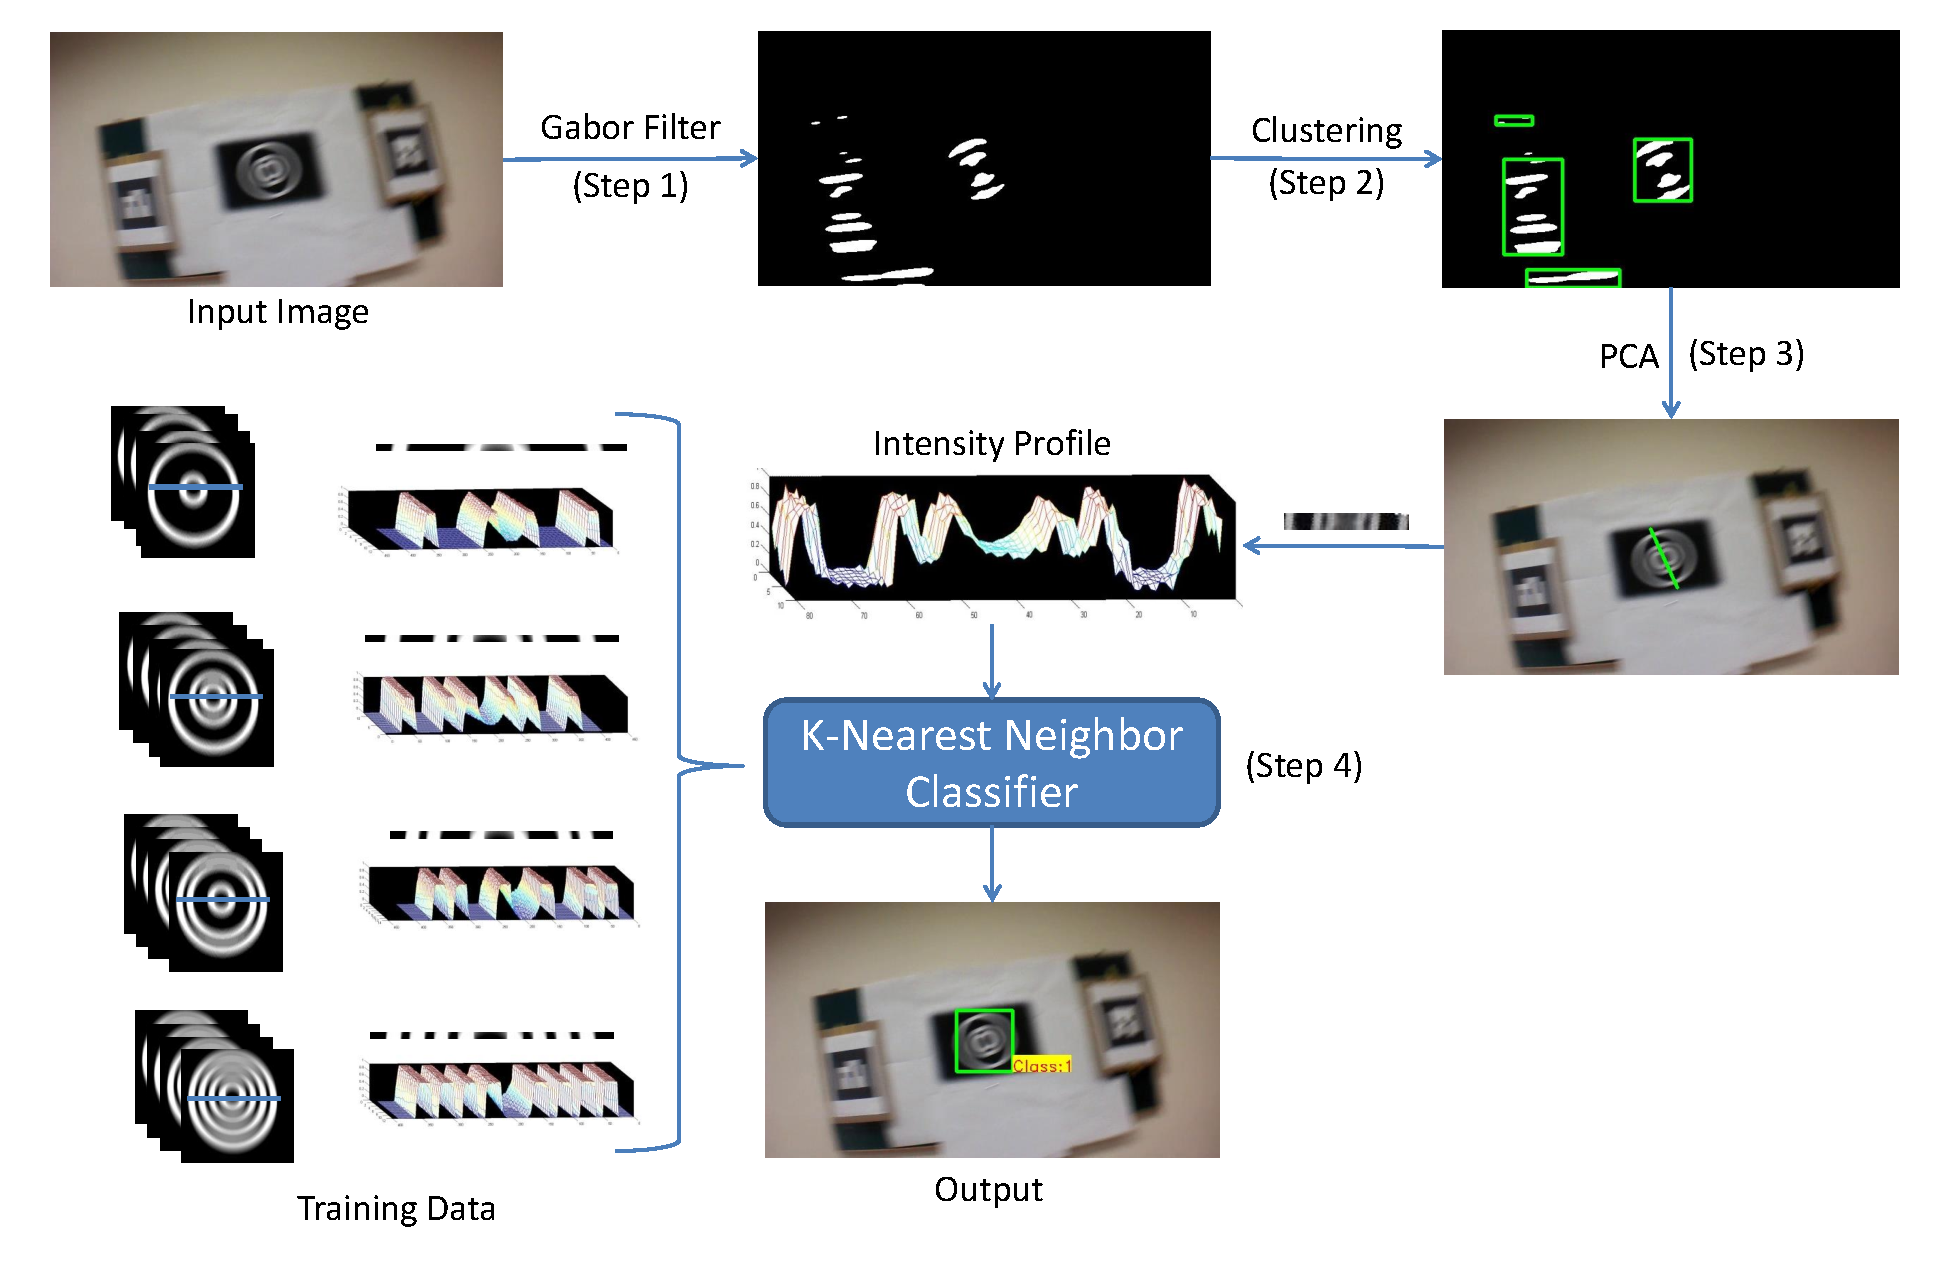
\includegraphics[width=\linewidth]{overall_flow.pdf}
\caption{Overall Workflow}
\end{figure}
Our fiducial detection strategy is different from \cite{NaimarkF02,Pitag13} and works
under significant amount of blur.   In particular, we assume that scene motion 
blur be modelled locally as a linear motion blur~\cite{}.  Under this assumption,
scene content perpendicular to the blur direction is unaffected by the blur.  Because
of our circular design, this means the perpendicular direction can be observed as a 
unblurred linear pattern.  Figure X shows an example with various motion directions.

Overall flow of fiducial detection algorithm can be summarised as follows:

\begin{itemize}
  \item Apply Gabor Filter on input image
  \item Find connected components in Gabor output
  \item Cluster the connected components into bounding boxes
  \item Detect code in the bounding box
  \begin{itemize}
    \item Run PCA on Gabor output in bounding box
    \item Find intensity profile along first principal component passing through
    centroid
    \item Classify the detected code by training examples
    standards.
  \end{itemize}
\end{itemize}

\textbf{Gabor Filter}: A 2D Gabor filter is a Gaussian kernel function modulated
by a sinusoidal plane wave. It is used to find high gradient patches from the
image. In our case, it will detect blur invariant sections of the fiducials. We
have applied Gabor filter for eight different orientations ($\theta = 0, 45,
90, 135, 180, 225, 270, 315$). We have used following parameters for
creating each Gabor kernel: $\lambda = 8$, $\gamma = 0.5$, $\sigma =
0.56\lambda$, $\psi = 0 \text(for real) = \pi/2 (for imaginary part)$. 
Then L2 norm of outputs along all orientations is calculated and finally, L2
normed image is binarized.

\begin{figure}
\centering
  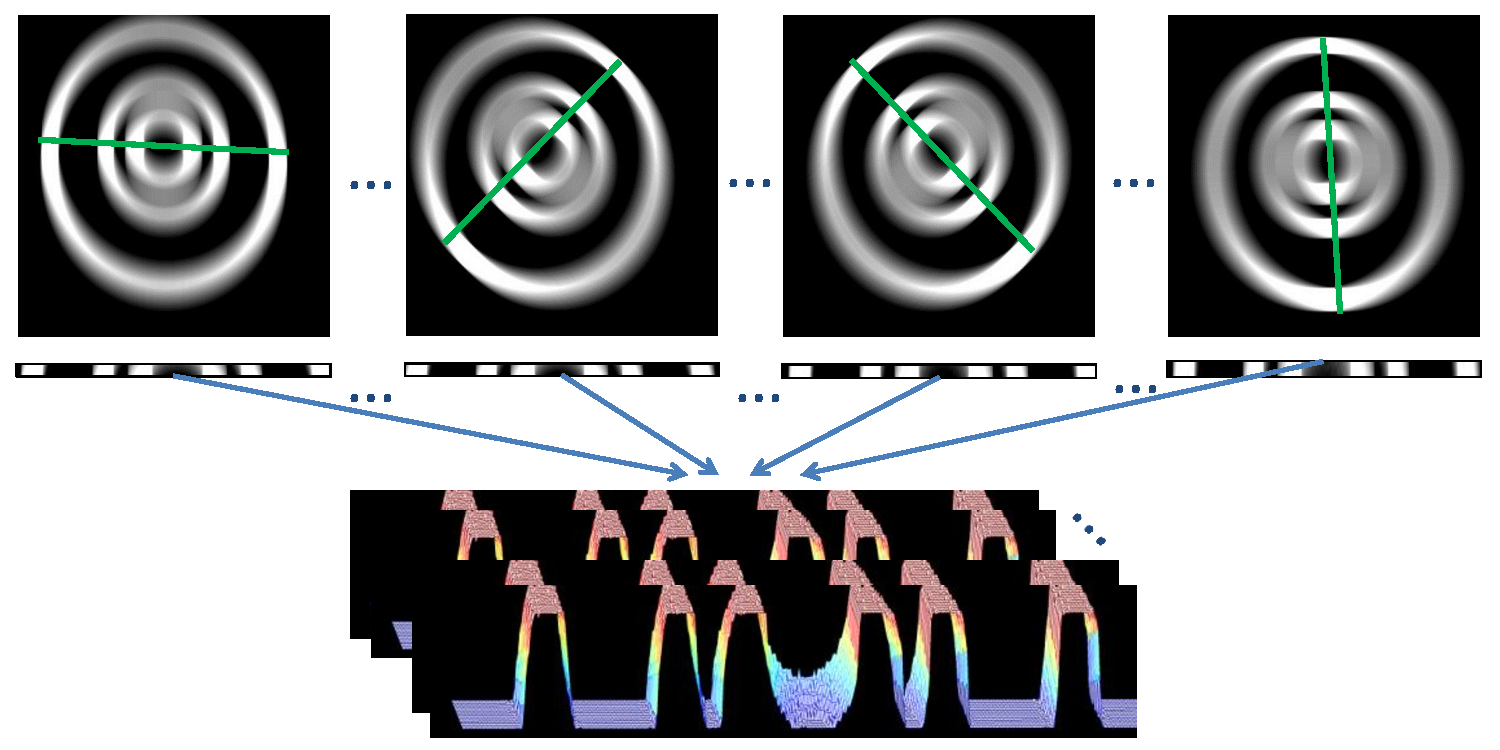
\includegraphics[width=\linewidth]{training_data.pdf}  
  \caption{Training data for the fiducial pattern with binary code ``01''}
\end{figure}

\textbf{Clustering}: Connected components are found from the Gabor output.
These connected components are then clustered in hierarchical fashion, to find
the group of closely positioned patches.

\textbf{PCA}: Principal Component Analysis is done on the clustered Gabor
output. Along first principal component, intensity profile in the original image
is found. Number of transitions in the intensity profile will give us the
number of rings.

\textbf{Classification}: Each synthetic fiducial pattern is blurred along 36
orientations (0, 10, 20, \ldots , 350) and intensity profile along first
principal component from every output is taken as training data for that
fiducial pattern. Test pattern is matched against training data using 
K-Nearest Neighbor Classifier (K=5) to output class label.

To increase classification accuracy, training data for patterns having same
number of rings is grouped together; e.g., in two bit binary coded fiducial,
training data for pattern ``01'' and ``10'' will be grouped together, In three
bit binary coded fiducial, training data for pattern “001”, “010” and “100” will
form one group while training data for pattern “110”, “011” and “101” will be
in other group, etc. Now, Depending on the number of detected rings in test
pattern, it is matched against corresponding group of training data, again
using  K-Nearest Neighbor Classifier. In this way, if we detect either zero
rings or maximum possible rings in the test pattern, there will be no need to do
further classification.

\section{Experimental Validation}

Our system has been tested on the image sequences captured from AR Drone
quadcopter. Each image sequence contains frames containing different fiducial
pattern. Sample output for each fiducial pattern is shown in Fig.
\ref{fig:output0} -- Fig. \ref{fig:output3}.

\begin{figure}
\begin{subfigure}{0.5\textwidth}
\centering
  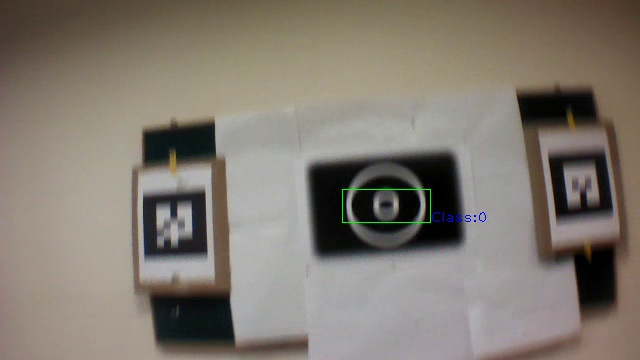
\includegraphics[width=\linewidth]{output_00.jpg}
  \caption{Binary code ``00''}
  \label{fig:output0}
\end{subfigure}
\begin{subfigure}{0.5\textwidth}
\centering
  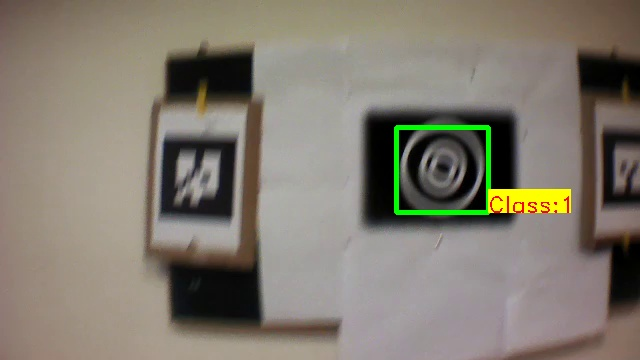
\includegraphics[width=\linewidth]{output_01.jpg}
  \caption{Binary code ``01''}
  \label{fig:output1}
\end{subfigure}
\begin{subfigure}{0.5\textwidth}
\centering
  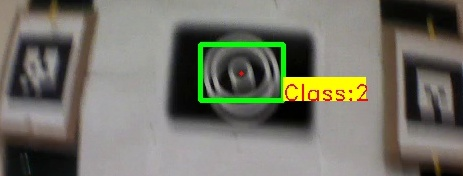
\includegraphics[width=\linewidth]{output_10.jpg}
  \caption{Binary code ``10''}
  \label{fig:output2}
\end{subfigure}
\begin{subfigure}{0.5\textwidth}
\centering
  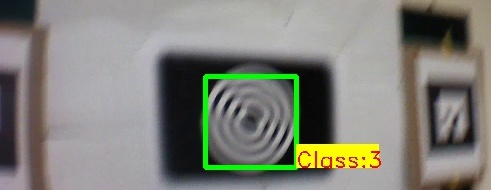
\includegraphics[width=\linewidth]{output_11.jpg}
  \caption{Binary code ``11''}
  \label{fig:output3}
  \end{subfigure}
  \caption{Sample Outputs for two bit binary coded fiducials}
\end{figure}

Our system has also been tested on images containing multiple fiducial patterns
in the same frame. Our algorithm successfully detected all fiducial patterns as
well as correctly classified them as shown in Fig. \ref{fig:output_all}
\begin{figure}
\centering
  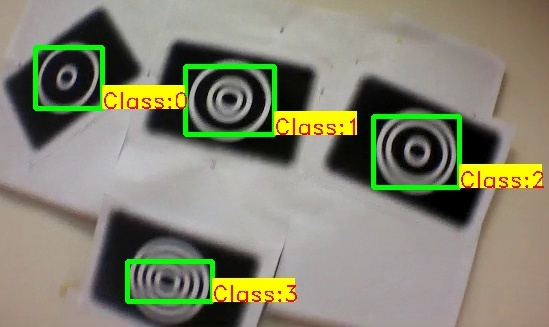
\includegraphics[width=.8\linewidth]{output_all_2.jpg}
  \caption{Sample output containing all two bit binary coded fiducial patterns}
  \label{fig:output_all}
\end{figure}

\subsection{Comparison}
We will compare our results with standard fiducials such as ARTag. Also, we will
compare our results with Blur driven tracker(BLUT)\cite{Wu:2011}.
\subsubsection{Comparison with ARTag}
First, we have repeated blur simulation experiment on our fiducials too, i.e.,
we have downsized our fiducial to size 150x150 and blurred it along various
orientations with different blur scales. Then, we tried to detect the patterns
using algorithm presented in earlier section. The comparison of recongition
rate is shown in Fig. \label{fig:recognition_rate}. 

\begin{figure}
\centering
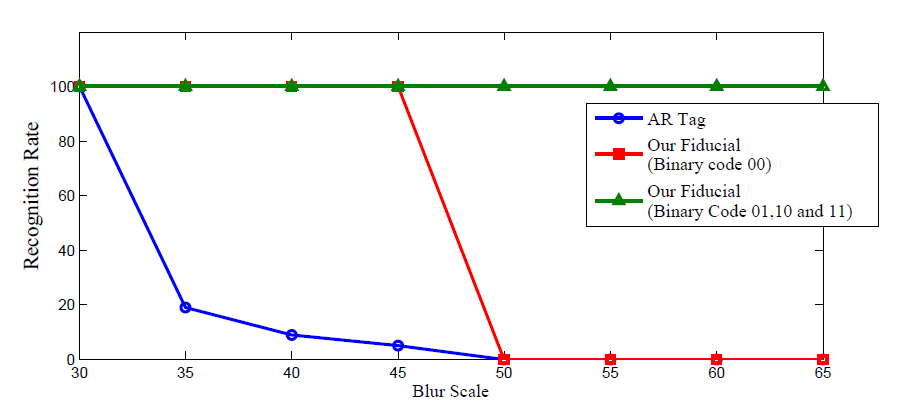
\includegraphics[width=\linewidth]{recognition_rate.png}
\caption{Comparison of recognition rate of AR Tag and our fiducials on
blur simulated data at various blur scales}
\label{fig:recognition_rate}
\end{figure}

Later, we recorded the real data using AR Drone quadcopter. In our experimental
setup, we have kept our fiducial alog with two AR Tags, to compare the
resilience of blur by each fiducial type. We have used ar\_track\_alvar, ROS
Wrapper for ALVAR libray \cite{ros_alvar}, to detect AR Tags from the stream
captured through quadcopter. The comparison of recognition rate shown in Table
\ref{tab:recongition_accuracy}. Classification accuracy of all fiducials(ARTag
as well as ours) is almost 100\%.

\begin{table}
\caption{Comparison of Recognition Rate of AR Tag and our fiducials on real
data captured through AR Drone}
\centering
\begin{tabularx}{0.8\textwidth}{|Y|Y|Y|Y|Y|}
\cline{1-5}
\multirow{2}{*}{AR Tag} & \multicolumn{4}{ c |}{Our Fiducial} \\ \cline{2-5}
& 00 & 01 & 10 & 11 \\  \cline{1-5}
65.6\% & 86.5\% & 94.1\% & 92.74\% & 93.54\% \\ \cline{1-5}
\end{tabularx}
\label{tab:recongition_accuracy}
\end{table}

\subsubsection{Comparison with BLUT} 
We have used sample image sequence to test the performance of BLUT\cite{Wu:2011}
and compare it with out result on the same image sequence. From Fig. \ref{fig:BLUT_output},
it can be inferred that BLUT is able to track the fiducial when the position of
fiducial doesnot change too much in successive frames. Also, it can be seen
that, once BLUT looses the track of the fiducial, it is not able to recover from
that. But, our algorithm is able to track the fiducial irrespecive of the change
in the position of the fiducial in the image as shown in Fig.
\ref{fig:our_output}.

\begin{figure}
\begin{subfigure}[b]{.19\textwidth}
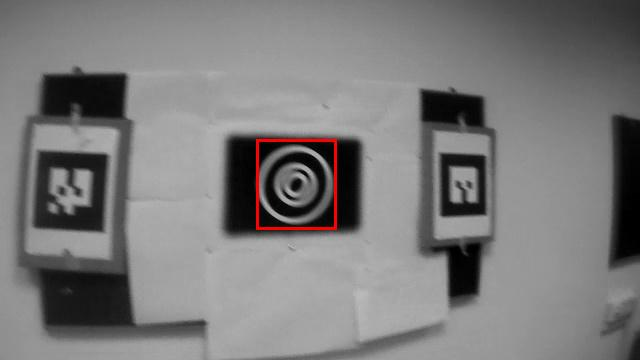
\includegraphics[width=\linewidth]{11.jpg}
\end{subfigure}
\begin{subfigure}[b]{.19\textwidth}
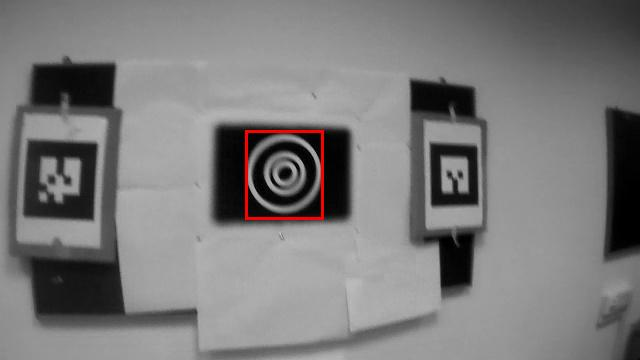
\includegraphics[width=\linewidth]{12.jpg}
\end{subfigure}
\begin{subfigure}[b]{.19\textwidth}
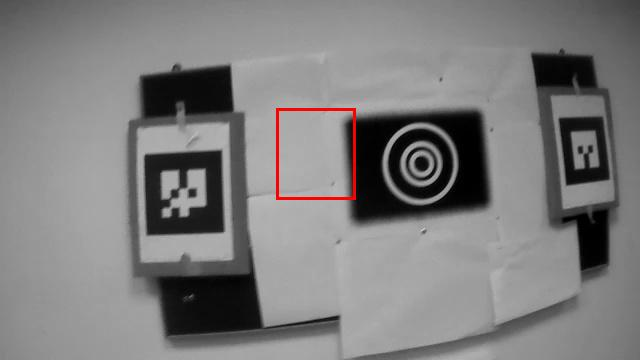
\includegraphics[width=\linewidth]{13.jpg}
\end{subfigure}
\begin{subfigure}[b]{.19\textwidth}
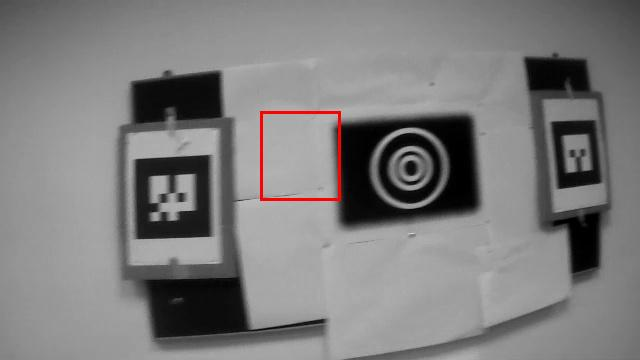
\includegraphics[width=\linewidth]{14.jpg}
\end{subfigure}
\begin{subfigure}[b]{.19\textwidth}
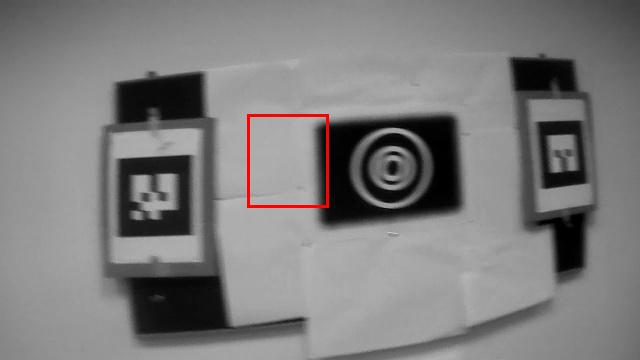
\includegraphics[width=\linewidth]{15.jpg}
\end{subfigure}
\caption{Output of BLUT on sample image sequence}
\label{fig:BLUT_output}
\end{figure}

\begin{figure}
\begin{subfigure}[b]{.19\textwidth}
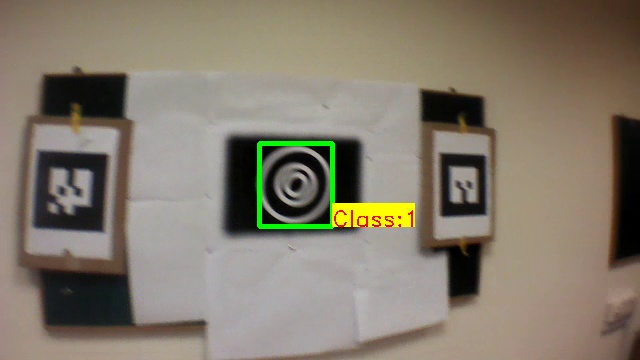
\includegraphics[width=\linewidth]{output11.jpg}
\end{subfigure}
\begin{subfigure}[b]{.19\textwidth}
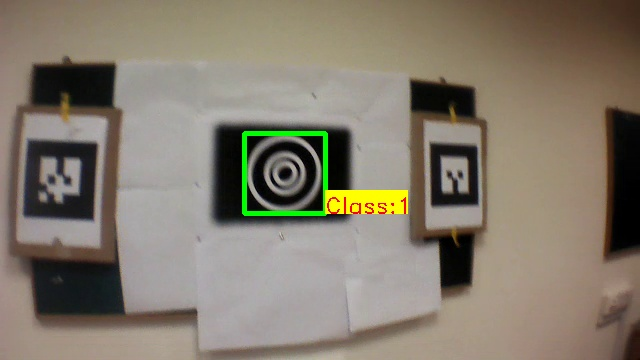
\includegraphics[width=\linewidth]{output12.jpg}
\end{subfigure}
\begin{subfigure}[b]{.19\textwidth}
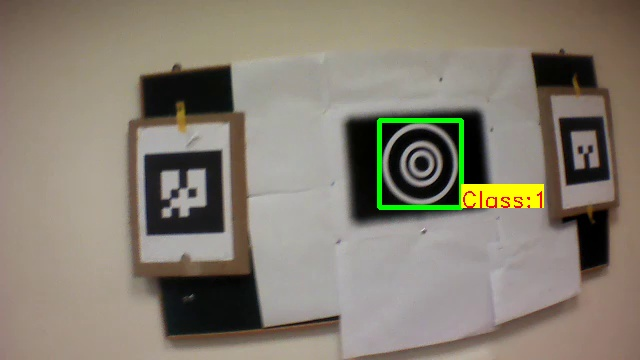
\includegraphics[width=\linewidth]{output13.jpg}
\end{subfigure}
\begin{subfigure}[b]{.19\textwidth}
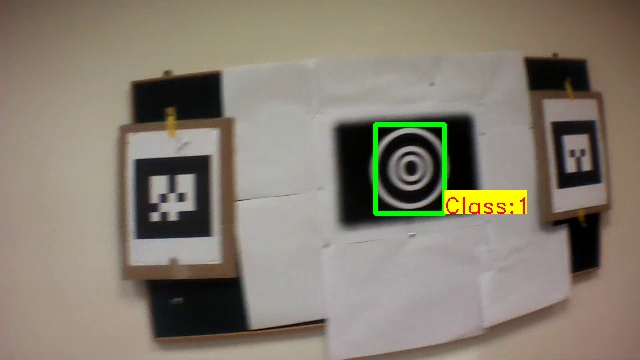
\includegraphics[width=\linewidth]{output14.jpg}
\end{subfigure}
\begin{subfigure}[b]{.19\textwidth}
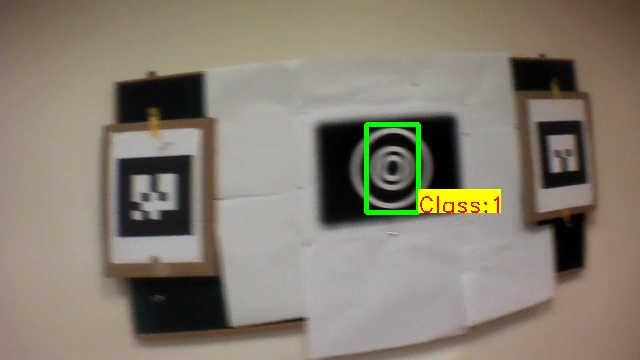
\includegraphics[width=\linewidth]{output15.jpg}
\end{subfigure}
\caption{Output of our algorithm on image sequence used in
Fig. \ref{fig:BLUT_output}}
\label{fig:our_output}
\end{figure}

\section{Discussion}
\begin{itemize}
\item Processing Time
\item False Positives and False Negatives
\item Pose Estimation
\end{itemize}
\section{Conclusion and Future Work}

\bibliographystyle{splncs}
\bibliography{egbib}

\end{document}

